\chapter{Architektura statku latającego typu tricopter}
\label{cha:architektura_statku_latajacego_typu_tricopter}

Poniższy rozdział przedstawia zbiór podstawowych zagadnień związanych z konstrukcją wirnikowca typu tricoper oraz zawiera informacje na temat zasad sterowania układem.

\section{Konstrukcja i sterowanie tricopterem}

Ze względu na skomplikowany sposób sterowania tricopterem w przestrzeni oraz złożoną konstrukcję, w poniższym podrozdziale zostaną przedstawione podstawowe zagadnienia związane z tym tematem.

Na rysunku \ref{fig:orientation} przedstawiono przyjętą konwencję nazewnictwa dla poszczególnych elementów tricoptera odpowiedzialnych za przemieszczanie się układu w przestrzeni. Pokazano również położenie modelu w układzie współrzędnych, które jest niezbędne do przejrzystego opisu zasad sterowania.

\begin{figure}[!htbp]
\centering
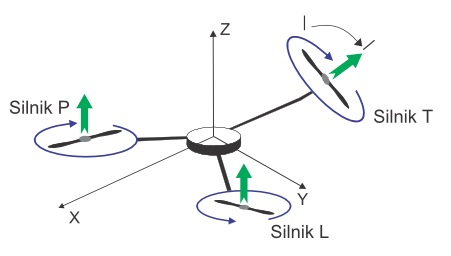
\includegraphics[width=0.7\linewidth]{./include/orientation}
\caption{Przyjęta orientacja tricoptera w układzie współrzędnych.}
\label{fig:orientation}
\end{figure}

Tricopter należy grupy rzadko spotykanych wielokomórkowców wyposażonych w nieparzystą liczbę silników odpowiadających za napędy w układzie.
Konstrukcja ta zdecydowanie utrudnia sterowanie ze względu na brak stabilności tego układu. Spowodowane jest to brakiem kompensacji siły bocznej pochodzącej od napędu niesparowanego. Skutkuje to autorotacją obiektu wokół osi Z przy założeniu, iż wszystkie wirniki są w pozycji pionowej, tak jak w przypadku większości obiektów latających pionowego startu. Aby wyeliminować powyższy efekt zastosowano odpowiedni moduł składający się z serwomechanizmu, który reguluje kąt nachylenia wirnika T.


Przemieszczanie obiektu latającego w przestrzeni wymaga opracowania metodyki sterowania poszczególnymi wirnikami podczas przemieszczania się względem każdej z osi.
Bazując na poprzednim algorytmie sterującym poniżej zaprezentowano sposoby przemieszczania względem konkretnych osi tricoptera. Szczegółowe informacje związane z powyższymi zagadnieniami zostały opisane w pracy inżynierskiej autora w rozdziale 5. %TODO zrobic odnosnik do inz

\subsection{Przemieszczanie względem osi X}
Aby dokonać obrotu względem osi X konieczna jest ingerencja w ciąg wirników L oraz P. Aby uzyskać efekt przechylenia w lewą stronę konieczna jest redukcja siły ciągu na silniku L. Opcjonalnie w celu przyśpieszenia manewru można proporcjonalnie zwiększyć ciąg silnika P. Na rysunku \ref{fig:axis_x} przedstawiono opisany manewr.

\begin{figure}[!htbp]
\centering
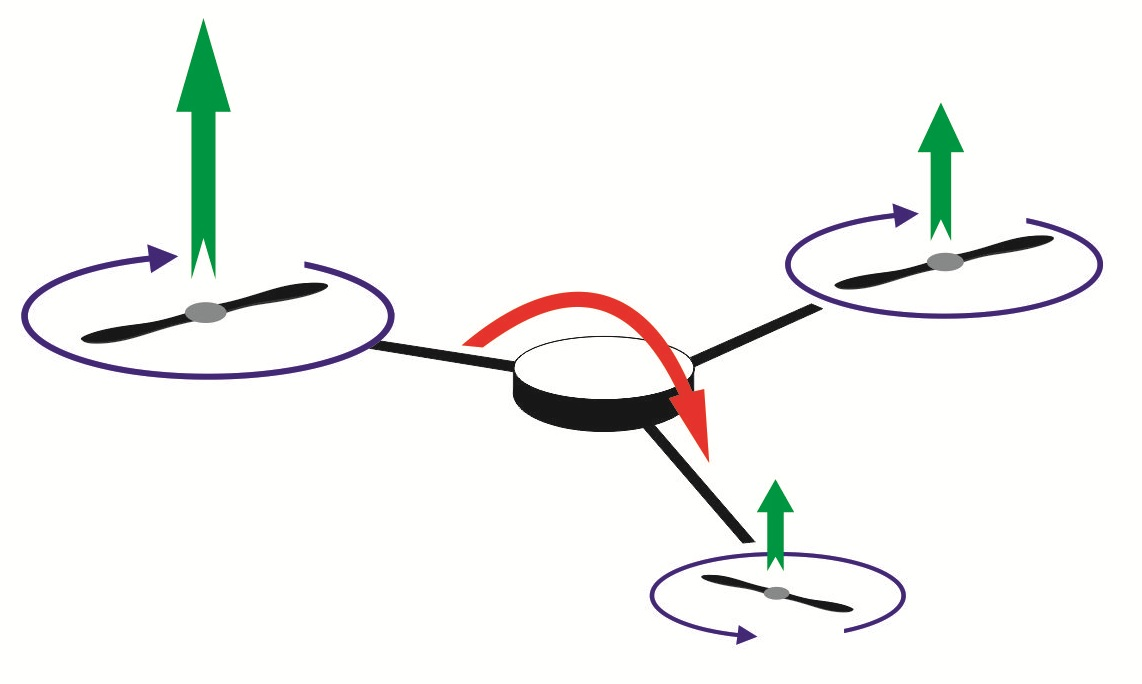
\includegraphics[width=0.7\linewidth]{./include/axis_x}
\caption{Sterowanie oraz stabilizacja w osi X.}
\label{fig:axis_x}
\end{figure}


\subsection{Przemieszczanie względem osi Y}
Obrót względem osi Y można zdecydowanie określić jako najważniejszy dla każdego obiektu latającego. Odpowiada on bowiem za przemieszczenie się w przód. Odchylenie tricoptera zapewnia się przez regulację ciągu na wirniku T. Tak jak w przypadku osi X można zwiększyć prędkość obrotu obiektu przez symetryczną modyfikacją mocy silników L oraz P wartość przeciwną co do znaku względem modyfikacji wirnika Z. Manewr ten został przedstawiony na rysunku \ref{fig:axis_y}.
\begin{figure}[!htbp]
\centering
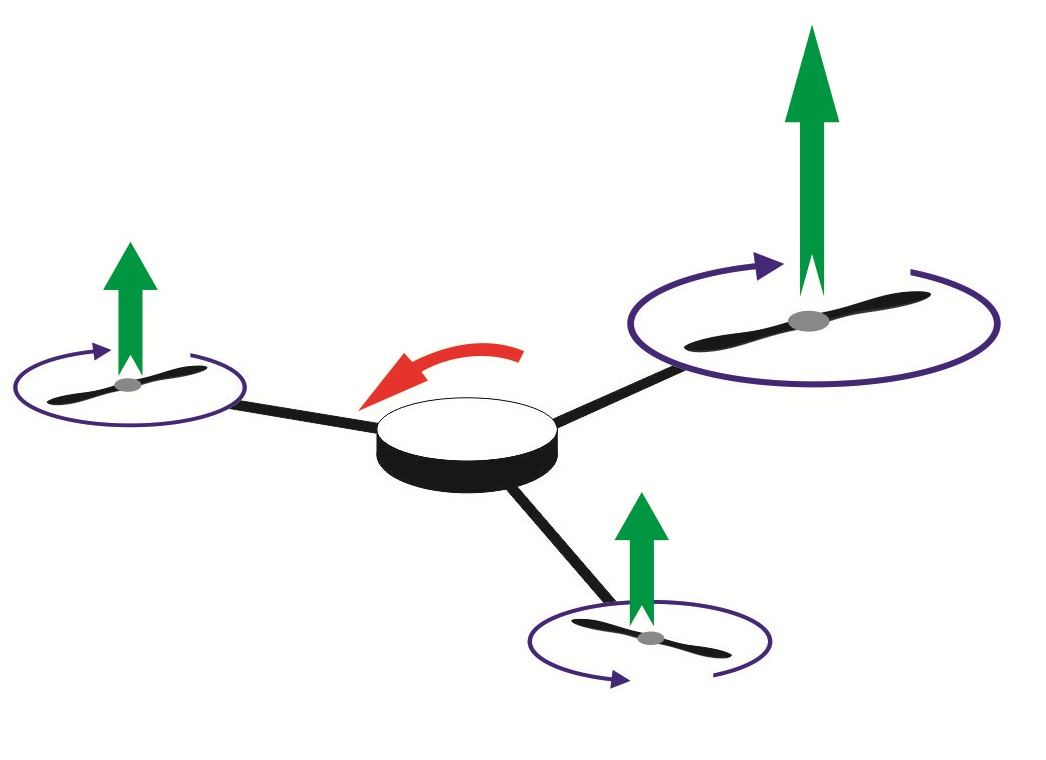
\includegraphics[width=0.7\linewidth]{./include/axis_y}
\caption{Sterowanie oraz stabilizacja w osi Y.}
\label{fig:axis_y}
\end{figure}


\subsection{Przemieszczanie względem osi Z}
Przemieszczanie względem osi Z jest głównie używane do zmiany kierunku lotu tricoptera. Manewr ten można wykonywać bez ingerencji w moc każdego z wirników. Zmiana kąta nachylenia silnika T powoduje pojawienie się efektu rotacji obiektu. Warto zwrócić uwagę, iż zbyt duże odchylenie wirnika od punktu stabilnego spowoduje również ruch tricoptera względem osi Y, ponieważ zmiana kąta nachylenia silnika Z powoduje zmianę pionowej siły ciągu, która odpowiada również za stabilizację tego obiektu. 

\begin{figure}[!htbp]
\centering
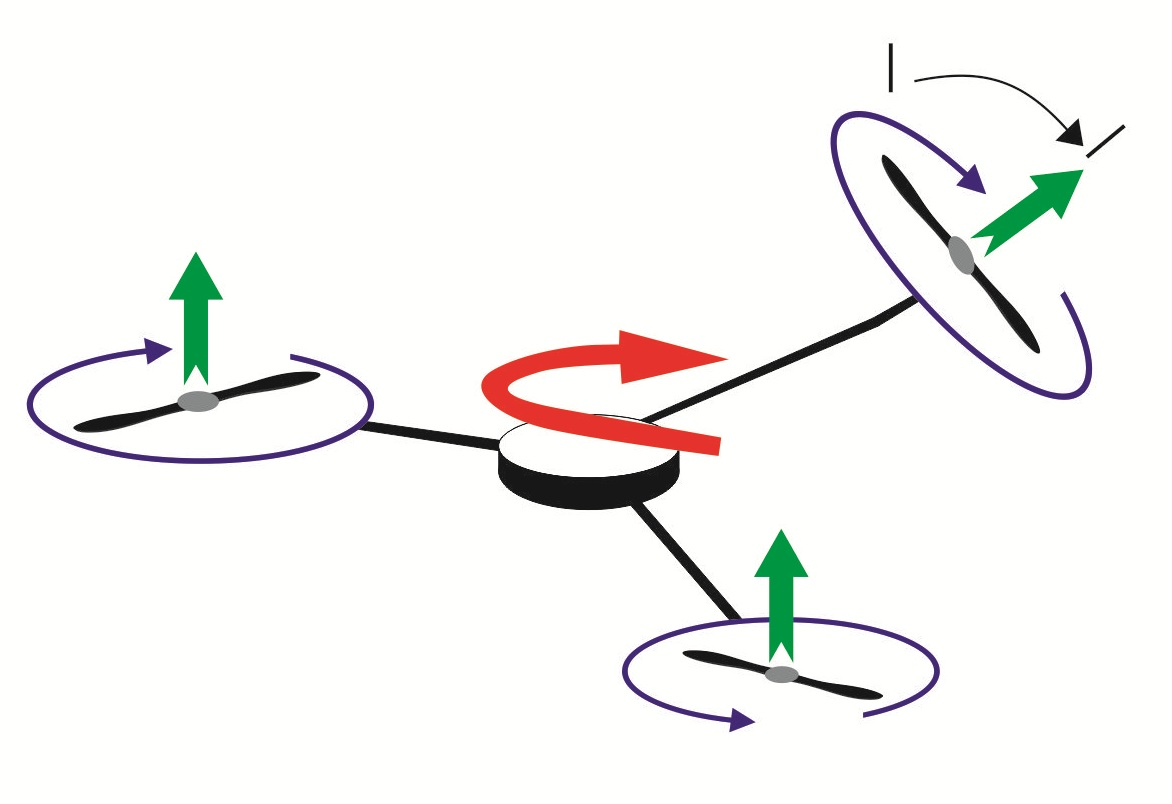
\includegraphics[width=0.7\linewidth]{./include/axis_z}
\caption{Sterowanie oraz stabilizacja w osi Z.}
\label{fig:axis_z}
\end{figure}


\section{Budowa modelu}
Ze względu na to, iż temat tej pracy bazuje na wykorzystaniu do testów gotowego obiektu latającego typu tricopter, autor zdecydował się pominąć szczegółowy opis budowy modelu. Na obrazku \ref{pic:tricopter} przedstawiono model wykorzystanego wielowirnikowca.

\begin{figure}[!htbp]
\centering
\includegraphics[width=0.7\linewidth]{./include/tricopter}
\caption{Model tricoptera.}
\label{pic:tricopter}
\end{figure}

Szczegółowe informacje dotyczące konstrukcji oraz parametrów wielowirnikowca zostały przedstawione w pracy inżynierskiej autora w rozdziale 2. %TODO odnośnik do inż.



